\documentclass[12pt,letterpaper]{article}
\renewcommand{\rmdefault}{phv}
\hbadness=99999

\usepackage[left=4cm,right=2cm,top=3cm,bottom=3cm]{geometry}
\usepackage[spanish,es-tabla]{babel}
\usepackage{fontenc}
\usepackage[utf8]{inputenc}
\usepackage{amsmath}
\usepackage{amssymb,amsfonts,cancel}
\usepackage{array}
\usepackage{enumerate}
\usepackage{etoolbox}
\usepackage{fancyhdr}
\usepackage{float}
\usepackage{graphicx}
\usepackage[pdfstartpage=1,backref=false,pagebackref=false,pdfborder={0 0 0},colorlinks=true,linkcolor=blue,citecolor=blue,urlcolor=blue]{hyperref}
\usepackage{longtable}
\usepackage{multicol}
\usepackage{multirow}
\usepackage{ragged2e}
\usepackage{caption}
\usepackage{subcaption}
\usepackage{titlesec}
\usepackage{titletoc}
\usepackage{titling}
\usepackage{colortbl}
\usepackage{xcolor}
\usepackage{tabularx}
\usepackage{listings}
\usepackage{booktabs}
\usepackage[round]{natbib}

% Configuración de encabezados y pies de página
\fancyhead{}
\fancyfoot[c]{\thepage}
\pagestyle{fancy}

% Configuración de tablas de contenido
\usepackage{tocloft}
\addto\captionsspanish{\renewcommand{\contentsname}{Contenido}}
\renewcommand{\cfttoctitlefont}{\hfill\normalsize}
\renewcommand{\cftaftertoctitle}{\hfill}
\renewcommand{\cftloftitlefont}{\hfill\normalsize}
\renewcommand{\cftafterloftitle}{\hfill\mbox{}}
\renewcommand{\cftlottitlefont}{\hfill\normalsize}
\renewcommand{\cftafterlottitle}{\hfill\mbox{}}

\renewcommand{\cftfigfont}{Fig. }
\renewcommand{\cfttabfont}{TABLA }
\renewcommand{\tablename}{TABLA}

\usepackage{layout}

% Formato de títulos
\titleclass{\subsubsubsection}{straight}[\subsection]
\newcounter{subsubsubsection}[subsubsection]
\renewcommand\thesubsubsubsection{\thesubsubsection.\arabic{subsubsubsection}}
\renewcommand\theparagraph{\thesubsubsubsection.\arabic{paragraph}}

\titleformat{\section}[block]{\bfseries\centering}{\thesection.}{1em}{}
\titleformat{\subsection}
{\normalfont\normalsize\bfseries\MakeUppercase}{\thesubsection}{1em}{}
\titlespacing*{\subsection}{0pt}{0em}{0em}
\titleformat{\subsubsection}
{\normalfont\normalsize\bfseries}{\thesubsubsection}{1em}{}
\titlespacing*{\subsubsection}{0pt}{0em}{0em}
\titleformat{\subsubsubsection}
{\normalfont\normalsize\bfseries}{\thesubsubsubsection}{1em}{}
\titlespacing*{\subsubsubsection}{0pt}{0em}{0em}

\makeatletter
\renewcommand\paragraph{\@startsection{paragraph}{5}{\z@}%
{0em}%
{-1em}%
{\normalfont\normalsize\bfseries}}
\renewcommand\subparagraph{\@startsection{subparagraph}{6}{\parindent}%
{0em}%
{-1em}%
{\normalfont\normalsize\bfseries}}
\def\toclevel@subsection{2}
\def\toclevel@subsubsection{3}
\def\toclevel@subsubsubsection{4}
\def\toclevel@paragraph{5}
\def\toclevel@subparagraph{6}
\setlength{\cftsecindent}{0pt}
\setlength{\cftsubsecindent}{0pt}
\setlength{\cftsubsubsecindent}{0pt}
\setlength{\cftfigindent}{0pt}
\setlength{\cfttabindent}{0pt}

\g@addto@macro\cftsecpagefont{\bfseries}
\g@addto@macro\cftsubsecpagefont{\bfseries\MakeUppercase}
\g@addto@macro\cftparapagefont{\bfseries}
\g@addto@macro\cftsubparapagefont{\bfseries}
\g@addto@macro\cftfigpagefont{\bfseries}
\g@addto@macro\cfttabpagefont{\bfseries}
\makeatother

\setcounter{secnumdepth}{4}
\setcounter{tocdepth}{4}

\makeatletter
\newcolumntype{U}{>{$}c<{$}}
\renewcommand{\fnum@table}{\textbf{\tablename~\thetable}.
\sffamily}
\renewcommand\thetable{\Roman{table}}
\makeatother

\renewcommand{\headrulewidth}{0pt}
\raggedbottom

\setlength{\arrayrulewidth}{1pt}
\setlength{\doublerulesep}{0mm}
\setlength{\parindent}{0em}
\setlength{\parskip}{2em}

% Colores y Listings
\definecolor{codegreen}{rgb}{0,0.6,0}
\definecolor{codegray}{rgb}{0.5,0.5,0.5}
\definecolor{codepurple}{rgb}{0.58,0,0.82}
\definecolor{backcolour}{rgb}{0.95,0.95,0.92}

\lstdefinestyle{pythonstyle}{
    backgroundcolor=\color{backcolour},
    commentstyle=\color{codegreen},
    keywordstyle=\color{magenta},
    numberstyle=\tiny\color{codegray},
    stringstyle=\color{codepurple},
    basicstyle=\ttfamily\footnotesize,
    breakatwhitespace=false,
    breaklines=true,
    captionpos=b,
    keepspaces=true,
    numbers=left,
    numbersep=5pt,
    showspaces=false,
    showstringspaces=false,
    showtabs=false,
    tabsize=2,
    language=Python,
    literate={á}{{\'a}}1 {é}{{\'e}}1 {í}{{\'i}}1 {ó}{{\'o}}1 {ú}{{\'u}}1 {Á}{{\'A}}1 {É}{{\'E}}1 {Í}{{\'I}}1 {Ó}{{\'O}}1 {Ú}{{\'U}}1 {ñ}{{\~n}}1 {Ñ}{{\~N}}1
}
\lstset{style=pythonstyle}

\begin{document}
    \definecolor{lightgray}{rgb}{0.75, 0.75, 0.75}

    \makeatletter
    \renewcommand{\fnum@figure}{\textbf{\figurename~\thefigure}. \sffamily}
    \renewcommand{\figurename}{\textbf{Fig.}}
    \makeatother

    \thispagestyle{empty}
    \begin{center}
        
\includegraphics[scale=1]{Figuras/horizontal-color}
    \end{center}
    \vspace{2.5cm}

    \textbf{DATOS GENERALES DEL ESTUDIANTE}
    \vspace{-0.5cm}

    \begin{tabularx}{\textwidth}{|>{\columncolor{lightgray}}l|X|}\hline
    \textbf{Nombre Estudiante} & Frank Edward Daza Gonzalez \\\hline
    \textbf{Programa Académico} & Maestría en Inteligencia Artificial y Ciencia de Datos \\\hline
    \textbf{Cédula} & 1144028994 \\\hline
    \textbf{Código Estudiantil} & 22500207 \\\hline
    \textbf{Correo} & frank\_edw.daza@uao.edu.co \\\hline
    \end{tabularx}

    \textbf{DATOS GENERALES DEL DIRECTOR}
    \vspace{-0.5cm}

    \begin{tabularx}{\textwidth}{|>{\columncolor{lightgray}}l|X|}\hline
    \textbf{Nombre Director} & Julian Hurtado López \\\hline
    \textbf{Correo} & jhurtado@uao.edu.co \\\hline
    \textbf{Nombre Codirector} &  \\\hline
    \textbf{Correo} &  \\\hline
    \end{tabularx}

    \textbf{DATOS DEL ANTEPROYECTO}

    \begin{longtable}{|p{\dimexpr\textwidth-2\tabcolsep-2\arrayrulewidth}|}
        \hline
        \rowcolor{lightgray}\centering\arraybackslash\textbf{TÍTULO DEL PROYECTO} \\\hline
        Diseño de una Arquitectura Híbrida CNN-VQC Ligera para el Diagnóstico de Tumores Cerebrales en Imágenes de Resonancia Magnética
        \\\hline
        \rowcolor{lightgray}\centering\arraybackslash\textbf{PALABRAS CLAVES/KEY WORDS} \\\hline
        Aprendizaje Automático Cuántico, QML, Transfer Learning, Eficiencia de Datos, RMI, Tumores Cerebrales \\\hline
        \rowcolor{lightgray}\centering\arraybackslash\textbf{RESUMEN} \\\hline
        El auge de las Redes Neuronales Convolucionales (CNN) ha revolucionado el diagnóstico médico asistido por computadora.
        Sin embargo, estas arquitecturas enfrentan un desafío crítico en medicina: la dependencia de grandes volúmenes de datos etiquetados (Big Data) para evitar el sobreajuste, un recurso a menudo escaso en entornos clínicos reales (\textit{Small Data}).
        Este proyecto investiga la viabilidad de una arquitectura híbrida cuántico-clásica para mitigar esta limitación.
        La propuesta integra una CNN clásica como extractora de características con un Clasificador Cuántico Variacional (VQC), aprovechando el \textit{Transfer Learning} para la clasificación multiclase de patologías cerebrales (glioma, meningioma, tumor pituitario).
        La metodología adopta un enfoque comparativo experimental. A diferencia de enfoques tradicionales centrados solo en la reducción de parámetros, este estudio contrastará el modelo híbrido frente a arquitecturas del estado del arte (EfficientNet, ResNet) evaluando específicamente la \textbf{capacidad de generalización en regímenes de pocos datos}.
        La hipótesis central anticipa que el componente cuántico, gracias a su alta expresividad en espacios de Hilbert, permitirá obtener métricas competitivas con fracciones reducidas del dataset de entrenamiento, demostrando una ventaja en eficiencia de datos sobre los modelos puramente clásicos.
        \\\hline
    \end{longtable}
    \setcounter{table}{0}

    \hypersetup{pageanchor=false}

    % PORTADA 1
    \newpage
    \thispagestyle{empty}
    \begin{center}
        \bfseries
        \MakeUppercase{Diseño de una Arquitectura Híbrida CNN-VQC Ligera para el Diagnóstico de Tumores Cerebrales en Imágenes de Resonancia Magnética}\\
        \vspace{4cm}
        
\includegraphics[scale=1.2]{Figuras/horizontal-color} \\
        \vspace{4cm}
        \MakeUppercase{FRANK EDWARD DAZA GONZALEZ}\\
        22500207\\
        \vfill
        UNIVERSIDAD AUTÓNOMA DE OCCIDENTE \\
        \MakeUppercase{FACULTAD DE INGENIERÍA Y CIENCIAS BÁSICAS} \\
        \MakeUppercase{PROGRAMA MAESTRÍA EN INTELIGENCIA ARTIFICIAL Y CIENCIA DE DATOS} \\
        SANTIAGO DE CALI \\
        2025
    \end{center}

    % PORTADA 2
    \newpage
    \thispagestyle{empty}
    \begin{center}
        \bfseries
        \MakeUppercase{Diseño de una Arquitectura Híbrida CNN-VQC Ligera para el Diagnóstico de Tumores Cerebrales en Imágenes de Resonancia Magnética}\\
        \vspace{2cm}
        
\includegraphics[scale=1.2]{Figuras/horizontal-color} \\
        \vspace{2cm}
        \MakeUppercase{FRANK EDWARD DAZA GONZALEZ}\\
        \vspace{2cm}
        Anteproyecto de grado para optar al título de\\
        Magíster en Inteligencia Artificial y Ciencia de Datos\\
        \vspace{2cm}
        Director\\
        \MakeUppercase{Julian Hurtado López}\\
        Doctor en Ingeniería\\
        \vfill
        UNIVERSIDAD AUTÓNOMA DE OCCIDENTE\\
        \MakeUppercase{FACULTAD DE INGENIERÍA Y CIENCIAS BÁSICAS}\\
        \MakeUppercase{PROGRAMA MAESTRÍA EN INTELIGENCIA ARTIFICIAL Y CIENCIA DE DATOS}\\
        SANTIAGO DE CALI\\
        2025
    \end{center}

    \clearpage
    \hypersetup{pageanchor=true}

    \makeatletter
    \renewcommand{\cftdotsep}{10000}
    \makeatother

    \setlength{\cftfigindent}{0pt}
    \setlength{\cfttabindent}{0pt}

    \newpage
    \noindent\renewcommand{\contentsname}{\textbf{CONTENIDO}}
    \vspace{-1cm}
    \addtocontents{toc}{\hfill \textbf{pág.} \par}
    {
        \hypersetup{linkcolor=black}
        \textbf{\tableofcontents}
    }

    \newpage
    \section*{INTRODUCCIÓN}
    \vspace{-0.5cm}
    \addcontentsline{toc}{section}{INTRODUCCIÓN}

    El diagnóstico por imagen es una piedra angular de la medicina moderna, siendo la Imagen por Resonancia Magnética (RMI, \textit{Magnetic Resonance Imaging}) la modalidad de referencia para la detección y caracterización de tumores cerebrales debido a su alto contraste en tejidos blandos.
    En la última década, la Inteligencia Artificial (IA), y específicamente el Aprendizaje Profundo (DL, \textit{Deep Learning}), ha transformado este campo, permitiendo el desarrollo de sistemas de diagnóstico asistido por computador (CAD, \textit{Computer-Aided Diagnosis}) con una precisión comparable a la de expertos humanos.
    Las Redes Neuronales Convolucionales (CNN, \textit{Convolutional Neural Networks}) se han establecido como la tecnología líder para estas tareas \citep{he2016deep}.
    Sin embargo, el despliegue efectivo de estos modelos enfrenta un obstáculo significativo: la ``paradoja de los datos''.
    Mientras que las arquitecturas de vanguardia (SOTA, \textit{State of the Art}) requieren millones de imágenes para ajustar sus parámetros sin caer en el sobreajuste (\textit{overfitting}), la disponibilidad de datos médicos etiquetados de alta calidad es intrínsecamente escasa y costosa de obtener \citep{litjens2017survey, willemink2020preparing, esteva2019guide}. Esta brecha limita la aplicabilidad de modelos masivos en patologías poco frecuentes o en centros médicos con bases de datos limitadas.

    El Aprendizaje Automático Cuántico (QML, \textit{Quantum Machine Learning}) emerge como una frontera prometedora para abordar este problema.
    En la actual era de dispositivos NISQ (\textit{Noisy Intermediate-Scale Quantum}), los modelos híbridos cuántico-clásicos proponen una sinergia innovadora: utilizar redes clásicas pre-entrenadas para la extracción de características robustas (Transfer Learning) y circuitos cuánticos variacionales (VQC) para el procesamiento final.
    La hipótesis subyacente sugiere que la alta expresividad de los circuitos cuánticos en espacios de Hilbert de alta dimensión podría permitir una mejor generalización con menos datos de entrenamiento que los clasificadores clásicos tradicionales \citep{mari2020transfer, abbas2021power}.

    Este proyecto propone el diseño y evaluación de una arquitectura híbrida VQC-CNN aplicada a la clasificación multiclase de tumores cerebrales.
    A diferencia de estudios previos enfocados únicamente en la reducción de parámetros, esta investigación busca establecer si el componente cuántico aporta una ventaja real en términos de \textbf{eficiencia de datos}.
    Se contrastará el modelo propuesto frente a arquitecturas clásicas optimizadas como EfficientNet \citep{tan2019efficientnet} bajo condiciones de escasez de datos, validando el potencial del QML para entornos médicos reales \citep{shahjalal2025hqcnn, khan2024brain}.

    \newpage
    \section{PLANTEAMIENTO DEL PROBLEMA}
    \vspace{-0.5cm}

    La clasificación automatizada de imágenes médicas mediante CNNs ha alcanzado hitos significativos.
    Autores seminales como \citet{he2016deep} sentaron las bases con arquitecturas profundas, las cuales, junto con variantes modernas optimizadas para RMI, han demostrado alta precisión.
    Sin embargo, el paradigma actual de ``más profundo es mejor'' conlleva desafíos críticos.
    La tendencia dominante ha sido el escalado masivo de modelos. Arquitecturas estándar como ResNet-50 contienen decenas de millones de parámetros.
    Si bien modelos más modernos como EfficientNet \citep{tan2019efficientnet} han optimizado la relación precisión-parámetros, persiste una barrera fundamental: el \textbf{Riesgo de Sobreajuste en Escenarios de Escasez de Datos}.

    El análisis de imágenes médicas se enfrenta a la disponibilidad limitada de conjuntos de datos.
    Entrenar modelos con millones de parámetros sobre datasets médicos pequeños (cientos o pocos miles de imágenes) conduce frecuentemente al sobreajuste, donde la red memoriza el ruido del entrenamiento en lugar de aprender características generalizables.
    Aunque técnicas clásicas como el aumento de datos (\textit{data augmentation}) mitigan esto parcialmente, no resuelven la ineficiencia estructural del aprendizaje clásico en regímenes de pocos datos (\textit{Few-Shot} o \textit{Low-Data regimes}).

    Aquí es donde el QML surge como una alternativa disruptiva.
    Teóricamente, los Circuitos Cuánticos Variacionales (VQC) pueden procesar información aprovechando el entrelazamiento y la superposición, lo que les otorga una mayor capacidad de representación (expresividad) por parámetro que las redes neuronales clásicas \citep{schuld2019feature}.
    Estudios recientes como los de \citet{shahjalal2025hqcnn} sugieren que esta ventaja teórica puede traducirse en rendimiento práctico en datasets médicos.
    Sin embargo, existe un vacío en la literatura experimental: ¿Se traduce esta ventaja teórica en un mejor rendimiento práctico cuando los datos son escasos?
    La mayoría de los estudios actuales comparan modelos cuánticos contra redes clásicas básicas, lo que infla la percepción de ventaja.
    Faltan evaluaciones rigurosas que contrasten las arquitecturas híbridas frente a modelos clásicos eficientes (como EfficientNet-B0) utilizando estrategias de \textit{Transfer Learning} en escenarios de datos limitados.

    \subsection{Pregunta de Investigación}
    \vspace{-0.5cm}
    ¿Puede una arquitectura híbrida cuántico-clásica, basada en Transfer Learning, demostrar una capacidad de generalización superior a la de arquitecturas clásicas del estado del arte (como EfficientNet-B0) en escenarios de entrenamiento con datos limitados, manteniendo métricas de precisión competitivas?

    \newpage
    \section{OBJETIVOS}
    \vspace{-0.5cm}

    \subsection{Objetivo General}
    \vspace{-0.5cm}
    Evaluar la viabilidad y eficiencia de una arquitectura híbrida cuántico-clásica para la clasificación multiclase de tumores cerebrales por medio de RMI, comparando su desempeño frente a arquitecturas clásicas en escenarios de escasez de datos.

    \subsection{Objetivos Específicos}
    \vspace{-0.5cm}
    \begin{enumerate}
        \item Desarrollar una arquitectura híbrida que integre una red neuronal clásica pre-entrenada (extractor de características) con un circuito cuántico variacional (VQC) optimizado utilizando técnicas de \textit{Angle Embedding} y \textit{Strongly Entangling Layers}.
        \item Entrenar los modelos de referencia clásicos: EfficientNet, ResNet con la base de datos seleccionada.
        % \item Comparar el desempeño de los modelos variando progresivamente el tamaño del conjunto de entrenamiento (ej. 10\%, 25\%, 50\%, 100\% de los datos) para evaluar la viabilidad y eficiencia de la propuesta cuántica.
        \item Comparar el desempeño y la eficiencia computacional de los modelos, variando progresivamente el tamaño del conjunto de entrenamiento e incluyendo métricas de tiempo para evaluar la viabilidad técnica de la propuesta.
    \end{enumerate}

    \newpage
    \section{JUSTIFICACIÓN Y ALCANCE}
    \vspace{-0.5cm}

    Este proyecto se justifica por la necesidad de democratizar el uso de IA en medicina, donde la recolección de ``Big Data'' no siempre es viable.
    Si se valida que los modelos híbridos aprenden mejor con menos datos, esto tendría un impacto directo en la capacidad de diagnosticar enfermedades raras o en la implementación de sistemas en hospitales pequeños.
   El proyecto aborda el problema desde la perspectiva del \textit{Hybrid Transfer Learning} \citep{mari2020transfer}.
    A diferencia de intentar entrenar redes cuánticas desde cero (lo cual sufre de problemas como ``Barren Plateaus''), el uso de redes pre-entrenadas permite aprovechar la potencia de la visión clásica y combinarla con la expresividad del espacio de características cuántico.
    Se busca evitar la generación de expectativas infundadas respecto a la supremacía cuántica actual, por el contrario, se busca cuantificar rigurosamente en qué nicho (específicamente \textit{Low-Data}) la tecnología NISQ actual puede ofrecer una ventaja tangible \citep{gupta2025systematic}.

    \textbf{Alcance:}
    \begin{enumerate}
        \item \textbf{Tarea:} Clasificación multiclase mediante RMI (4 clases: glioma, meningioma, pituitario, no tumor).
        No se aborda la segmentación.
        \item \textbf{Datos:} Uso exclusivo de datasets públicos de imágenes de RM, garantizando la reproducibilidad \citep{nickparvar2023dataset}.
        \item \textbf{Enfoque Experimental:} Validación cruzada entrenando con fracciones del dataset total para simular escasez de datos.
        \item \textbf{Tecnología:} Implementación en simuladores cuánticos integrados con PyTorch. No se requiere hardware cuántico real, enfocándose en la validación algorítmica y de arquitectura.
    \end{enumerate}

Independientemente del resultado experimental, este proyecto garantiza: 
\begin{itemize}
    \item \textbf{Contribución metodológica:} Protocolo reproducible de evaluación 
de HQCNN en régimen de datos limitados
    \item \textbf{Contribución empírica:} Caracterización cuantitativa de trade-offs 
accuracy-tiempo-parámetros
    \item \textbf{Contribución práctica:} Guía basada en evidencia sobre cuándo 
considerar (o no) soluciones QML en diagnóstico médico.
\end{itemize}

\newpage
\section{ANTECEDENTES Y ESTADO DEL ARTE}
\vspace{-0.5cm}

La investigación en QML ha transitado hacia aplicaciones prácticas mediante modelos híbridos.
    \citet{lusnig2024leveraging} demostraron eficacia en clasificación de hígado graso. Sin embargo, el estado del arte presenta desafíos.
    Muchos estudios utilizan CNNs muy simples (ej. 2 capas) como comparativa, lo cual es una línea base débil.
    Estudios recientes sugieren que la verdadera ventaja del QML a corto plazo no está en la velocidad, sino en la \textbf{Generalización}.
    Modelos como HQCNN \citep{shahjalal2025hqcnn} han demostrado superioridad sobre ResNet en MedMNIST, pero raramente se comparan contra un \textit{Fine-tuned EfficientNet} en igualdad de condiciones de datos restringidos.
    Este proyecto busca llenar ese vacío experimental.

    \newpage
    \section{MARCO TEÓRICO}
    \vspace{-0.5cm}

    El marco teórico de esta investigación se articula sobre la convergencia de dos paradigmas computacionales: el Aprendizaje Profundo (\textit{Deep Learning}) para el procesamiento de imágenes y el Cómputo Cuántico Variacional (VQC). A continuación, se fundamentan los principios matemáticos y arquitectónicos que sustentan la propuesta de una red híbrida eficiente.

    \subsection{Deep Learning y Eficiencia Computacional}
    \vspace{-0.5cm}
    Las Redes Neuronales Convolucionales (CNN) constituyen el estado del arte en tareas de visión por computador. Su arquitectura se inspira en la organización del córtex visual biológico y se basa matemáticamente en la operación de convolución discreta. Dada una imagen de entrada $I$ y un filtro (kernel) $K$ de dimensiones $(2k+1) \times (2k+1)$, el mapa de características $S$ en la posición $(i, j)$ se define como:
    \begin{equation}
        S(i, j) = (I * K)(i, j) = \sum_{m=-k}^{k} \sum_{n=-k}^{k} I(i+m, j+n) K(m, n)
    \end{equation}
    Esta operación permite la extracción de características locales (bordes, texturas) con invarianza a la traslación, reduciendo drásticamente el número de parámetros respecto a las redes totalmente conectadas (MLP). Sin embargo, la demanda de precisión ha llevado a un escalado masivo de estos modelos.

    \subsubsection{Arquitecturas de Referencia: El Reto del Escalado}
    \vspace{-0.5cm}
    Para contextualizar la eficiencia, se analizan dos familias de arquitecturas clave en la literatura:
    \begin{itemize}
        \item \textbf{ResNet (Residual Networks):} Introducida por \citet{he2016deep}, esta arquitectura resolvió el problema de la degradación del gradiente en redes profundas mediante la introducción de "conexiones residuales". Estas permiten que el flujo de información salte capas ($x_{l+1} = F(x_l) + x_l$), facilitando el entrenamiento de modelos muy profundos (ej. ResNet-50, ResNet-101), aunque a costa de un alto número de parámetros.
        \item \textbf{EfficientNet:} Propuesta por \citet{tan2019efficientnet}, representa el estado del arte en eficiencia clásica. Los autores demostraron que existe una relación óptima entre la profundidad ($\alpha$), el ancho ($\beta$) y la resolución ($\gamma$) de la red. Mediante un método de "Escalado Compuesto" (\textit{Compound Scaling}), EfficientNet-B0 logra un rendimiento superior a ResNet-50 con una reducción de parámetros de orden de magnitud ($\approx 5.3$ millones), sirviendo como el \textit{baseline} clásico más exigente para esta investigación.
    \end{itemize}

    \begin{figure}[H]
        \centering
        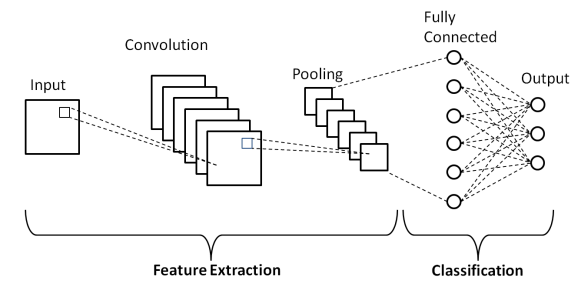
\includegraphics[width=0.8\textwidth, height=5cm, keepaspectratio]{Figuras/General structure of a Convolutional Neural Network and the concept of.png}
        \caption{Estructura general de una Red Neuronal Convolucional y el concepto de convolución.}
        \label{fig:cnn_structure}
    \end{figure}

    \subsection{Fundamentos de Cómputo Cuántico Aplicado (QML)}
    \vspace{-0.5cm}
    El Quantum Machine Learning (QML) aprovecha las propiedades de la mecánica cuántica para el procesamiento de información. La unidad fundamental es el \textbf{qubit}, que se representa como un vector unitario en un espacio de Hilbert complejo bidimensional ($\mathbb{C}^2$):
    \begin{equation}
        |\psi\rangle = \alpha|0\rangle + \beta|1\rangle, \quad \text{donde } |\alpha|^2 + |\beta|^2 = 1
    \end{equation}
    La ventaja computacional potencial reside en la capacidad de procesar información en un espacio de estados que crece exponencialmente ($2^N$) con el número de qubits $N$, permitiendo representar distribuciones de datos complejas que son intratables para modelos clásicos.

    \subsubsection{Circuitos Cuánticos Variacionales (VQC)}
    \vspace{-0.5cm}
    En la era actual NISQ (\textit{Noisy Intermediate-Scale Quantum}), los algoritmos dominantes son los variacionales. Un VQC es un circuito cuántico parametrizado $U(\theta)$ que funciona de manera análoga a una red neuronal:
    \begin{enumerate}
        \item \textbf{Codificación de Datos (Embedding):} Es el paso crítico de mapear datos clásicos $\mathbf{x}$ a un estado cuántico $|\psi_{\mathbf{x}}\rangle$. Según \citet{qml_data_encoding_2022}, la elección del embedding determina la expresividad del modelo. Este proyecto utilizará principalmente \textit{Angle Embedding}, donde las características de entrada rotan los qubits en la esfera de Bloch ($R_x(x_i)$), debido a su eficiencia en circuitos de baja profundidad.
        \item \textbf{Ansatz Variacional:} Es la estructura del circuito compuesta por compuertas de rotación con parámetros entrenables $\theta$ y compuertas de entrelazamiento (como CNOTs). La calidad del \textit{Ansatz} define la capacidad del modelo para explorar el espacio de Hilbert y encontrar la solución óptima \citep{anzatz_vqc_2024}.
        \item \textbf{Medición:} Finalmente, se mide el valor esperado de un observable (generalmente el operador Pauli-Z, $\langle Z \rangle$) para colapsar el estado cuántico a un valor escalar clásico que pueda ser interpretado por la función de pérdida.
    \end{enumerate}

    \begin{figure}[H]
        \centering
        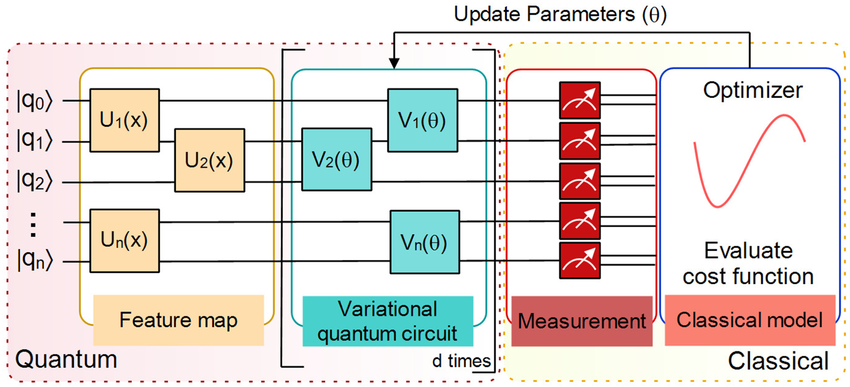
\includegraphics[width=0.8\textwidth, height=5cm, keepaspectratio]{Figuras/VQC Scheme- Coding, Variational Analysis and Measurement.png}
        \caption{Esquema de un VQC: Codificación, Ansatz Variacional y Medición.}
        \label{fig:vqc_scheme}
    \end{figure}

    \subsection{Transferencia de Aprendizaje Híbrido (Hybrid Transfer Learning)}
    \vspace{-0.5cm}
    El modelo propuesto se basa en el esquema de \textit{Quantum Transfer Learning} formalizado por \citet{mari_qtl_2020}. En este enfoque, una red clásica pre-entrenada actúa como extractor de características, reduciendo la alta dimensionalidad de las imágenes de RM a un vector de características compacto. Este vector sirve como entrada para el VQC, que actúa como la capa clasificadora final ("Quantum Head").

    Para entrenar este sistema híbrido de extremo a extremo (\textit{end-to-end}), es necesario calcular el gradiente de la función de costo con respecto a los parámetros cuánticos. Esto se logra mediante la "Regla de Cambio de Parámetros" (\textit{Parameter Shift Rule}), que permite evaluar el gradiente exacto de un circuito cuántico ejecutándolo con parámetros desplazados, integrándose así con el mecanismo de autogradiente de PyTorch \citep{bergholm2018pennylane}.

    % \newpage
    % \section{DISEÑO METODOLÓGICO}
    % \vspace{-0.5cm}

    % Para el cumplimiento del objetivo general de esta propuesta, se contempla el desarrollo de tres objetivos específicos, con los que se busca dar respuesta al problema identificado. Como principio metodológico se propone la revisión constante de la literatura desde el inicio hasta su culminación. A continuación, se presenta cada objetivo específico con sus respectivas actividades

    % \subsection{Fase 1: Revisión Y Selección De Datos}
    % Se utilizará el ``Brain Tumor MRI Dataset'' \citep{nickparvar2023dataset} disponible en repositorios públicos.
    % Este dataset contiene 7,023 imágenes balanceadas en 4 clases, ideal para \textit{benchmarking}.
    % Se aplicará preprocesamiento estándar (redimensionamiento, normalización) para garantizar la compatibilidad de los datos.

    % \subsection{Fase 2: Diseño de Arquitecturas}
    % \begin{itemize}
    %     \item \textbf{Clásica (Baseline):} EfficientNet-B0 con una capa densa final (clasificador).
    %     \item \textbf{Híbrida (Propuesta):} EfficientNet-B0 (con capas congeladas o fine-tuning parcial) conectada a una capa cuántica (\textit{TorchLayer} de PennyLane) que actúa como clasificador final.
    %     La salida de la CNN se reducirá a $n$ características que serán codificadas mediante \textit{Angle Embedding}.
    % \end{itemize}

    % \subsection{Fase 3: Experimentación en Escenarios de Datos}
    % Esta es la fase crítica.
    % Se entrenarán ambos modelos en los siguientes subconjuntos de datos (estratificados):
    % \begin{itemize}
    %     \item 10\% del dataset de entrenamiento.
    %     \item 25\% del dataset de entrenamiento.
    %     \item 50\% del dataset de entrenamiento.
    %     \item 100\% del dataset de entrenamiento.
    % \end{itemize}

    % \subsection{Fase 4: Evaluación}
    % Comparación de curvas de aprendizaje (Accuracy/Loss) y métricas finales (F1-Score, Recall) en el conjunto de prueba (que se mantiene fijo).
    % Se busca identificar el punto de cruce donde el modelo híbrido podría superar al clásico.

    % \subsection{Resultados Esperados}
    % Se espera observar que, a medida que disminuye la cantidad de datos disponibles, la degradación del rendimiento en el modelo híbrido sea menor que en el modelo clásico, evidenciando una mayor robustez.



    \newpage
    \section{DISEÑO METODOLÓGICO}
    \vspace{-0.5cm}
    
    La metodología propuesta se fundamenta en un enfoque experimental comparativo, estructurado en tres fases que corresponden directamente a los objetivos específicos del proyecto. Cada fase desglosa actividades críticas necesarias para validar la hipótesis de eficiencia de datos en arquitecturas híbridas.
    
    \subsection{Fase 1: Desarrollo de la Arquitectura Híbrida CNN-VQC (Objetivo Específico 1)}
    Esta fase técnico-constructiva tiene como fin diseñar el modelo híbrido que combine la potencia de la visión por computadora clásica con la expresividad del cómputo cuántico.
    
    \begin{itemize}
        \item \textbf{A1. Configuración del Extractor de Características:} Se seleccionará la arquitectura \textit{EfficientNet-B0} pre-entrenada con \textit{ImageNet}. Se procederá a la congelación de las capas convolucionales para actuar como un extractor de mapas de características fijos, reduciendo la salida final a un espacio latente de baja dimensionalidad compatible con el número de qubits disponibles.
        \item \textbf{A2. Diseño del Clasificador Cuántico Variacional (VQC):} Se implementará en la librería \textit{PennyLane} un circuito cuántico parametrizado. Esta actividad incluye la definición del método de \textit{Angle Embedding} para mapear las características clásicas en ángulos de rotación de los qubits, y el diseño de un \textit{Ansatz} basado en \textit{Strongly Entangling Layers} para maximizar la capacidad de representación del modelo.
        \item \textbf{A3. Implementación de la Interfaz Híbrida:} Mediante el módulo \textit{TorchLayer}, se integrará el circuito cuántico como la capa final de clasificación dentro del flujo de tensores de \textit{PyTorch}, permitiendo el entrenamiento mediante el algoritmo de \textit{backpropagation} clásico y la regla de cambio de parámetro (\textit{Parameter Shift Rule}) para los gradientes cuánticos.
    \end{itemize}
    
    
    
    \subsection{Fase 2: Establecimiento de Líneas Base y Preparación de Datos (Objetivo Específico 2)}
    Esta fase garantiza que la comparación sea estadísticamente válida al establecer el rendimiento máximo que los modelos tradicionales pueden alcanzar con el conjunto de datos completo.
    
    \begin{itemize}
        \item \textbf{A4. Curaduría y Auditoría del Dataset:} Se validarán las 7,023 imágenes del \textit{Brain Tumor MRI Dataset}, realizando un análisis de balanceo de clases para asegurar que el entrenamiento no presente sesgos hacia categorías predominantes (ej. no tumor vs. glioma).
        \item \textbf{A5. Pipeline de Preprocesamiento y Aumento:} Se diseñará un flujo de transformación que incluya redimensionamiento a 224x224 píxeles, normalización estadística y técnicas de \textit{Data Augmentation} (rotaciones leves y \textit{flips}) para fortalecer la robustez de los modelos clásicos de referencia.
        \item \textbf{A6. Benchmark Clásico (SOTA):} Se entrenarán modelos \textit{EfficientNet-B0} y \textit{ResNet-50} utilizando el 100\% del dataset. Estos resultados servirán como el límite superior de precisión contra el cual se contrastará la eficiencia del modelo cuántico en condiciones de escasez de datos.
    \end{itemize}
    
    \subsection{Fase 3: Evaluación de Generalización en Escenarios de Escasez de Datos (Objetivo Específico 3)}
    Fase crítica orientada a medir la ventaja cuántica en términos de eficiencia de aprendizaje con pocos ejemplos (\textit{Small Data}).
    
    \begin{itemize}
        \item \textbf{A7. Definición de Escenarios de Escasez:} Creación de subconjuntos de datos estratificados al 10\%, 25\% y 50\% del total del dataset.
        \item \textbf{A8. Ejecución de Pruebas de Estrés y Rigor Estadístico:} Se realizarán $n$ ejecuciones independientes (ej. $n=5$) para cada configuración de modelo y tamaño de dataset. Esto permitirá capturar la variabilidad del entrenamiento y garantizar la reproducibilidad de los hallazgos.
        \item \textbf{A9. Evaluación Multimétrica:} Además de las métricas de clasificación (Accuracy, F1-Score), se registrará sistemáticamente el \textbf{tiempo de entrenamiento y latencia de inferencia} para discutir la viabilidad del modelo híbrido en comparación con los baselines clásicos.
        \item \textbf{A10. Análisis Estadístico de Resultados:} Se aplicarán pruebas de \textbf{Análisis de Varianza (ANOVA)} para determinar si las diferencias de desempeño observadas entre la arquitectura HQCNN y los modelos clásicos son estadísticamente significativas, permitiendo una conclusión científica robusta sobre la ventaja cuántica.
    \end{itemize}
    
    \subsection{Cronograma de Actividades}
    La ejecución de las fases y actividades descritas se proyecta en un periodo de ocho meses (2025), permitiendo tiempos adecuados para la iteración algorítmica y la experimentación computacional.
    
    \begin{table}[H]
        \centering
        \small
        \begin{tabularx}{\textwidth}{|X|c|c|c|c|c|c|c|c|}
        \hline
        \rowcolor{lightgray} \centering \textbf{Actividad / Mes (2026)} & \textbf{1} & \textbf{2} & \textbf{3} & \textbf{4} & \textbf{5} & \textbf{6} & \textbf{7} & \textbf{8} \\ \hline
        \multicolumn{9}{|l|}{\cellcolor{lightgray!50}\textbf{Fase 1: Arquitectura}} \\ \hline
        A1. Configuración Extractor & \cellcolor{blue!20}X & & & & & & & \\ \hline
        A2. Diseño VQC & \cellcolor{blue!20}X & \cellcolor{blue!20}X & \cellcolor{blue!20}X & & & & & \\ \hline
        A3. Integración Híbrida & & & \cellcolor{blue!20}X & \cellcolor{blue!20}X & & & & \\ \hline
        \multicolumn{9}{|l|}{\cellcolor{lightgray!50}\textbf{Fase 2: Benchmarking}} \\ \hline
        A4. Auditoría Dataset & \cellcolor{blue!20}X & & & & & & & \\ \hline
        A5. Pipeline Preprocesado & & \cellcolor{blue!20}X & & & & & & \\ \hline
        A6. Entrenamiento Baselines & & & & \cellcolor{blue!20}X & \cellcolor{blue!20}X & & & \\ \hline
        \multicolumn{9}{|l|}{\cellcolor{lightgray!50}\textbf{Fase 3: Experimentación}} \\ \hline
        A7. Estratificación Escenarios & & & & & \cellcolor{blue!20}X & & & \\ \hline
        A8. Pruebas de Estrés ($n=5$) & & & & & & \cellcolor{blue!20}X & \cellcolor{blue!20}X & \\ \hline
        A9. Registro de Tiempos & & & & & & & \cellcolor{blue!20}X & \cellcolor{blue!20}X \\ \hline
        A10. Análisis ANOVA & & & & & & & & \cellcolor{blue!20}X \\ \hline
        \end{tabularx}
        \caption{Cronograma de actividades actualizado con rigor estadístico y múltiples baselines.}
        \label{tab:cronograma}
    \end{table}









    

    \newpage
    \section{RECURSOS Y ASPECTOS ECONÓMICOS}
    \vspace{-0.5cm}

    \begin{tabularx}{\textwidth}{|p{0.25\textwidth}|X|}
        \hline
        {\textbf{TIPO DE RECURSO}} & \textbf{DESCRIPCIÓN} \\
        \hline
        Capital Humano & \textbf{Estudiante investigador:} Frank Edward Daza Gonzalez.\\
        \hline
        Tecnologías Blandas & \textbf{Software:} Python, PyTorch, PennyLane.
        \newline
        \textbf{Herramientas:} Repositorios de datos públicos (Kaggle).
        \newline
        \textbf{Metodología:} Diseño experimental cuantitativo.
        \\
        Tecnologías Duras & Equipo de cómputo personal y servicios de nube (Google Colab) para simulación de circuitos cuánticos y entrenamiento de redes neuronales.
        \\
        \hline
        \hline
        Infraestructura & No se requiere laboratorio físico.
        Trabajo remoto/local. \\
        \hline
        Financieros & Financiación propia.
        Uso de recursos de acceso libre. \\
        \hline
    \end{tabularx}

    \newpage
    \renewcommand{\refname}{REFERENCIAS}
    \addcontentsline{toc}{section}{REFERENCIAS}
    \bibliographystyle{apalike}
    \bibliography{Referencias}

\end{document}